\chapter{طراحی یگ پلتفرم \lr{MLOps}}
 
\section{مقدمه}
در این بخش می خواهیم مقدمه ای از طراحی و هدف آن بنویسیم

\section{مدیریت سیستم}
\subsection{خط لوله \lr{CI/CD}}

در دنیای فناوری اطلاعات، زیرساخت‌های تغییرناپذیر\footnote{\lr{Immutable Infrastructure}} و تغییرپذیر\footnote{\lr{Mutable Infrastructure}} دو رویکرد مهم در مدیریت و نگهداری سیستم‌ها هستند. زیرساخت‌های تغییرناپذیر به سیستم‌هایی اشاره دارند که پس از ایجاد، بدون تغییر باقی می‌مانند و در صورت نیاز به تغییر، سیستم های جدید جایگزین آنها می‌شوند. این رویکرد با مزایایی همچون کاهش پیچیدگی‌های مدیریتی، افزایش قابلیت پیش‌بینی و کاهش ریسک‌های مرتبط با تغییرات ناخواسته همراه است \cite{DevopsIaac2}. به کمک ابزارهایی مانند داکر و کوبرنتیز، پیاده‌سازی زیرساخت‌های تغییرناپذیر امکان‌پذیر است و از قابلیت مقیاس‌پذیری بالایی برخوردارند. سیستم‌های ابری غالباً از روش تغییرناپذیر استفاده کرده تا از مزایای آن بهره‌مند شوند. در مقابل، زیرساخت‌های تغییرپذیر به سیستم‌هایی اشاره دارند که می‌توانند به طور پویا تغییر کنند و تنظیمات و پیکربندی‌های جدید را بپذیرند. این رویکرد، انعطاف‌پذیری بیشتری را فراهم می‌کند و برای محیط‌هایی که نیاز به تغییرات مکرر دارند، مناسب‌تر است. با این حال، مدیریت تغییرات در زیرساخت‌های تغییرپذیر ممکن است چالش‌های بیشتری از جمله افزایش ریسک خطاها و نیاز به نظارت مداوم به همراه داشته باشد. انتخاب بین این دو رویکرد به نیازها و اولویت‌های سازمان بستگی دارد. در حالی که زیرساخت‌های تغییرناپذیر برای محیط‌های تولید با نیاز به ثبات و قابلیت پیش‌بینی بالا مناسب‌ترند، زیرساخت‌های تغییرپذیر برای محیط‌های توسعه و آزمایش که نیاز به انعطاف‌پذیری دارند، کاربرد بیشتری دارند \cite{DevopsIaac1}. 

با افزایش استفاده از سیستم‌های ابری و رویکرد تغییرناپذیر، مفهوم \lr{GitOps} معرفی شده است که از گیت برای مدیریت زیرساخت و پیکربندی بهره می‌برد. \lr{GitOps} توسط \lr{Weaveworks} در سال ۲۰۱۷ معرفی شد که رویکردی مدرن برای پیاده سازی خط لوله \lr{CD} بر روی سیستم های ابری است. در حالی که ابزارهای سنتی تحویل مداوم عمدتاً از مدل \lr{Push} استفاده می‌کنند، \lr{GitOps} مدل \lr{Pull} را معرفی می‌کند که به خصوص با کانتینرها و پیکربندی‌های اعلامی به خوبی کار می‌کند و آن را به یک روند محبوب در اکوسیستم بومی ابر تبدیل کرده است  \cite{Devopsgitops}. از معروف ترین ابزار کلیدی که فرآیندهای \lr{GitOps} را تسهیل می‌کند می توان به \lr{ArgoCD} اشاره کرد. 

\begin{figure}[t]
	\centering
	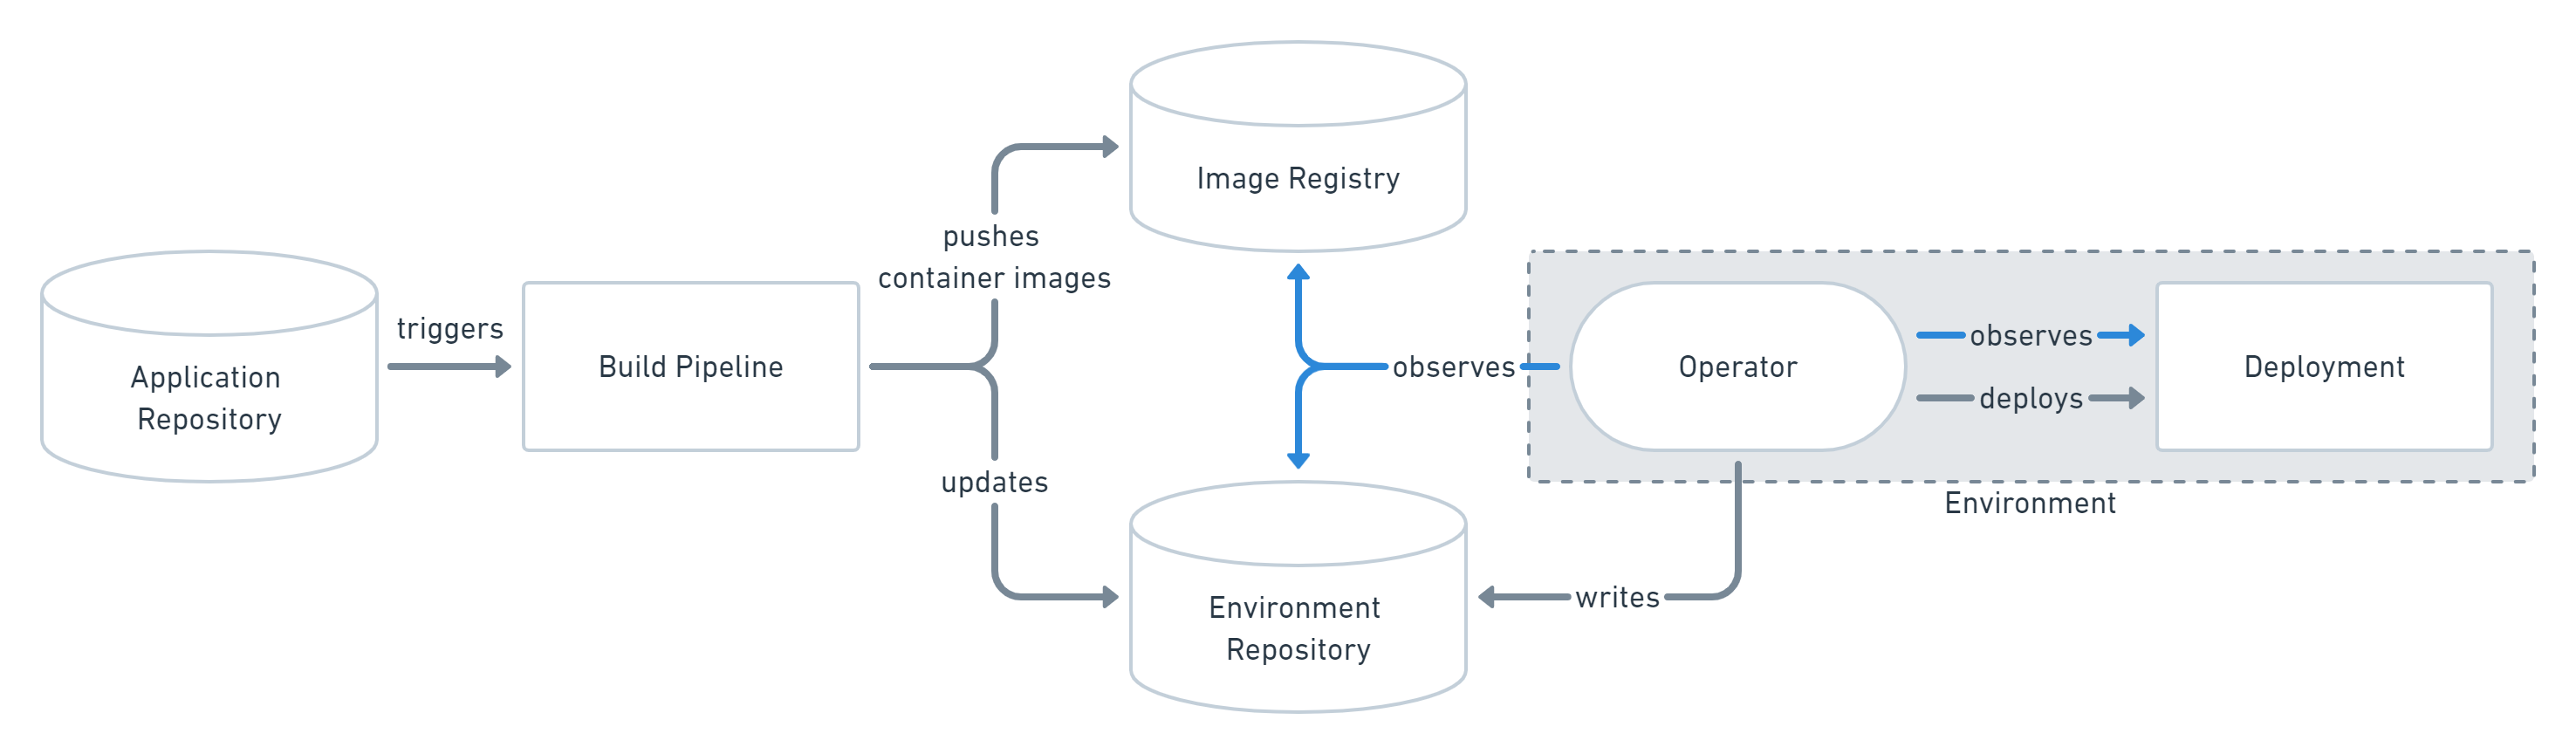
\includegraphics[scale=0.15]{gitops-pull.png}
	\caption{استقرار مبتنی بر \lr{Pull}}
	\label{fig: gitops pull}
\end{figure}

همان طور که گفته شد دو رویکرد در پیاده سازی خط لوله \lr{CD} وجود دارد. در مدل \lr{Pull} 
(شکل 
~\ref{fig: gitops pull})
مانند \lr{GitOps}، توسعه‌دهندگان حالت مطلوب را در مخزن گیت قرار می دهند. ابزاری نظیر \lr{ArgoCD} در محیط تولید به صورت خودکار این تغییرات را شناسایی کرده و اعمال می‌کنند. این مدل امنیت را افزایش می‌دهد زیرا نیازی به اعتبارنامه‌های دسترسی مستقیم برای توسعه‌دهندگان نیست. هم چنین این مدل مشکل استقرارهای مبتنی بر \lr{Push} را حل می کند، که در آن محیط تنها زمانی به روز می شود که مخزن محیط به روز شود. 
در مقابل، در مدل \lr{Push} (شکل 
~\ref{fig: gitops push})، استقرار در محیط تولید شامل خطوط لوله \lr{CI/CD} با اسکریپت‌هایی است که با هر تغییر در گیت فعال می‌شوند. این اسکریپت‌ها معمولاً ساخت، تست و در نهایت استقرار برنامه‌ها یا تنظیم پیکربندی‌های جدید در محیط تولید را با استفاده از ابزارهای خط فرمان و اعتبارنامه‌های ارائه شده انجام می‌دهند. این مدل کنترل دقیق‌تر بر فرآیند استقرار، اعمال سریع تغییرات، انعطاف‌پذیری بالا در مدیریت سناریوهای پیچیده و پشتیبانی بهتر از تغییرات جزئی را فراهم می‌کند، که در محیط‌های متنوع و پویا بسیار مفید است \cite{Devopsgitops}.
\begin{figure}[t]
	\centering
	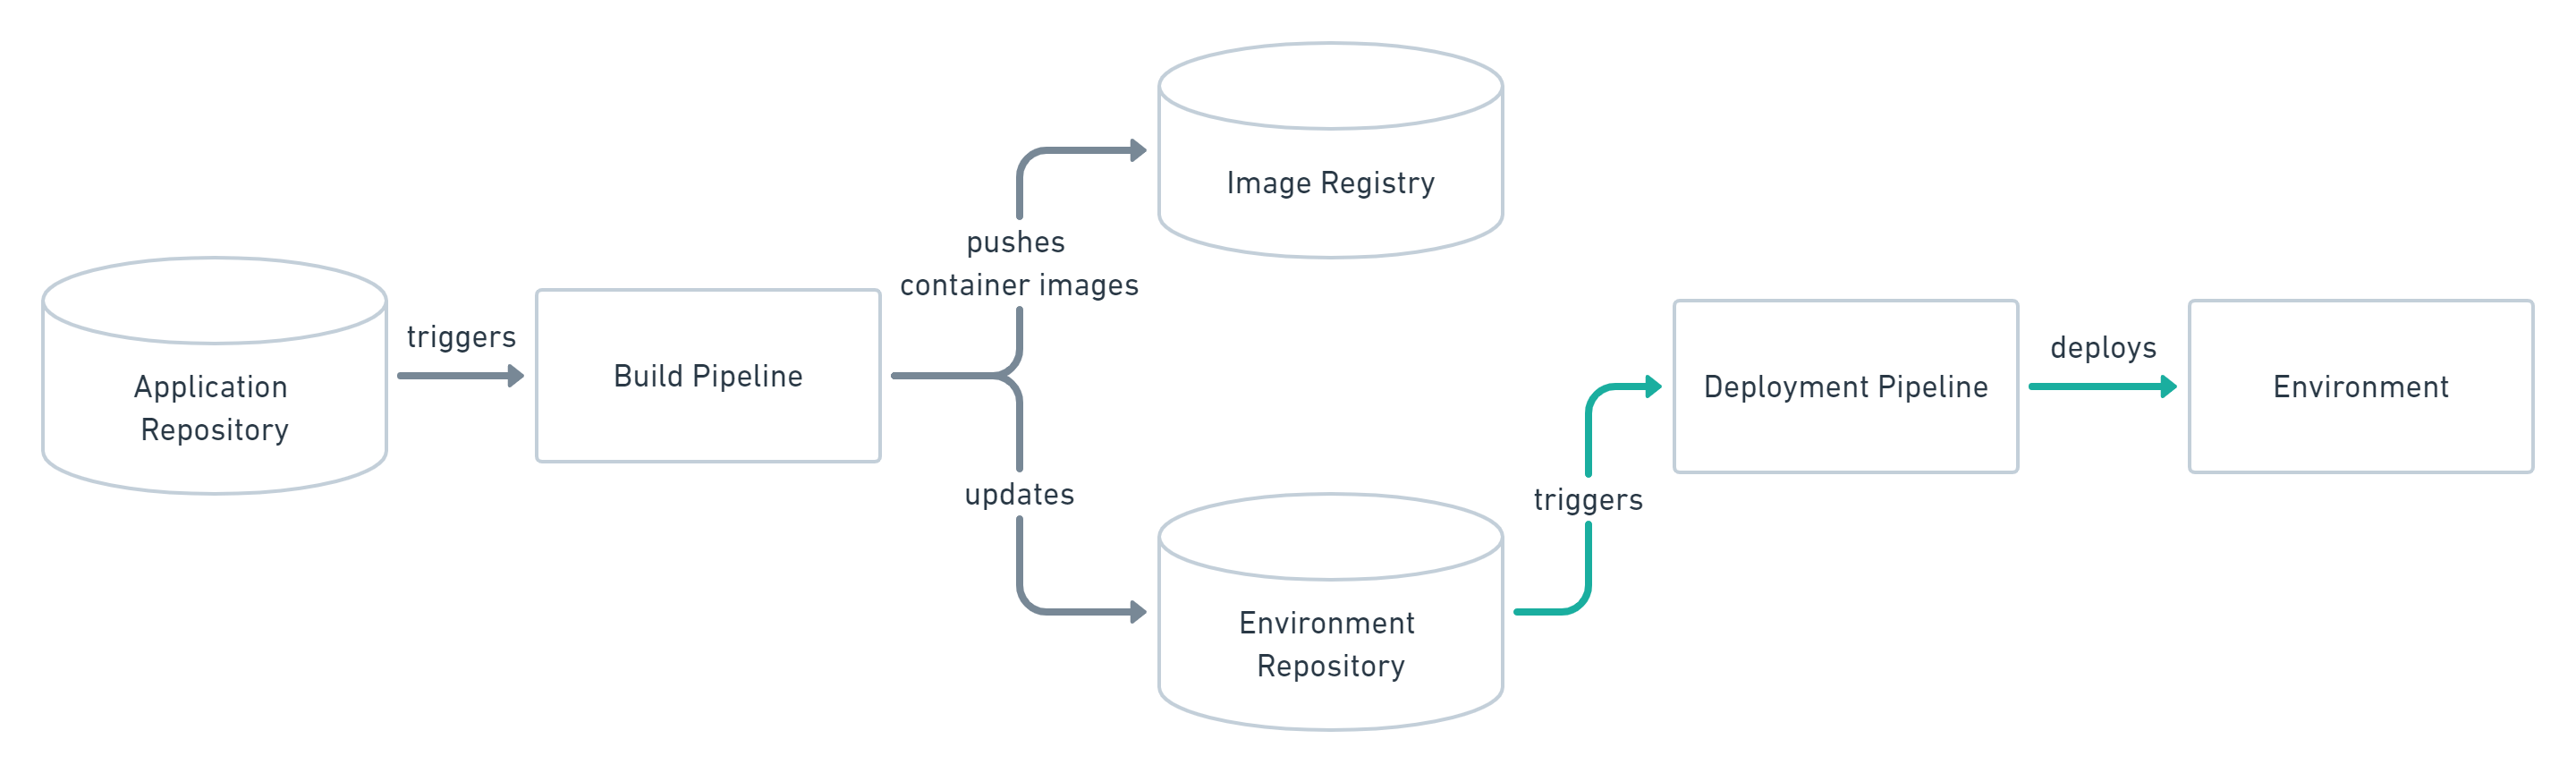
\includegraphics[scale=0.15]{gitops-push.png}
	\caption{استقرار مبتنی بر \lr{Push}}
	\label{fig: gitops push}
\end{figure}

به منظور پیاده‌سازی یک ابزار متن‌باز برای مدیریت خط لوله های \lr{CI/CD} که برای سیستم‌های ابری نیز مناسب باشد،  رویکرد تغییرپذیر  به همراه استراتژی استقرار مبتنی بر \lr{Push} انتخاب شده است. انتخاب رویکرد تغییرپذیر به دلیل نیاز به انعطاف‌پذیری بیشتر در محیط‌هایی که تغییرات مکرر و به‌روزرسانی‌های سریع دارند، انجام شده است. زیرساخت‌های تغییرپذیر به ما امکان می‌دهند تا به سرعت به تغییرات نیازمندی‌ها، پاسخ دهیم و تنظیمات و پیکربندی‌های جدید را به راحتی اعمال کنیم. این ویژگی در محیط‌های توسعه و آزمایش بسیار حیاتی است، زیرا تغییرات مداوم و آزمایش‌های متعدد بخشی از فرآیند توسعه نرم‌افزار هستند. هم چنین روش \lr{Push} نیز به دلیل سادگی و کارایی در اعمال به‌روزرسانی‌ها انتخاب شده است. با استفاده از این روش، می‌توانیم به‌روزرسانی‌ها را مستقیماً به سرورها ارسال کنیم و اطمینان حاصل کنیم که تمام سیستم‌ها به سرعت و بدون نیاز به مداخله دستی به‌روز می‌شوند. این رویکرد همچنین به کاهش زمان مورد نیاز برای انتشار تغییرات کمک می‌کند. در این راستا، \lr{Jenkins} به عنوان ابزار پیاده‌سازی و مدیریت خط لوله \lr{CI/CD} انتخاب شده است. جنکینز به دلیل متن‌باز بودن و دارا بودن تعداد زیادی پلاگین، انعطاف‌پذیری بسیار بالایی دارد و می‌تواند با انواع سیستم‌های ابری و رویکردهای زیرساختی سازگار شود. جنکینز همچنین با \lr{Ansible} که به عنوان ابزار مدیریت پیکربندی انتخاب شد، به خوبی سازگار است. این ترکیب به ما اجازه می‌دهد تا پیکربندی‌های پیچیده را به سادگی مدیریت کنیم و اطمینان حاصل کنیم که تمام زیرساخت‌ها به صورت هماهنگ عمل می‌کنند.

\subsection{مخزن کد منبع}

مخزن کد منبع\footnote{\lr{Source Code Repository}} یک سیستم ذخیره‌سازی و مدیریت کد است که به توسعه‌دهندگان این امکان را می‌دهد تا به صورت مشترک و هماهنگ بر روی پروژه‌های نرم‌افزاری کار کنند. این مخازن ابزارهای متعددی را برای تسهیل و بهبود فرآیند توسعه نرم‌افزار فراهم می‌کنند. یکی از اصلی‌ترین ویژگی های مخزن کد منبع، کنترل نسخه است که به توسعه‌دهندگان این امکان را می‌دهد تا تغییرات کد را پیگیری کرده و به نسخه‌های قبلی بازگردند. این ابزارها با ثبت تاریخچه تغییرات و شاخه‌بندی، امکان مدیریت همزمان چندین ویژگی یا رفع اشکال را فراهم می‌کنند بدون اینکه تغییرات یکدیگر را تحت تأثیر قرار دهند.

رایج‌ترین و پرکاربردترین این مخازن، گیت است که با ابزارهای مختلفی مانند \lr{GitHub}، \lr{GitLab} و \lr{Bitbucket} یکپارچه می‌شود. از آنجایی که یکی از شرط های پیاده سازی پلتفرم، متن باز بودن ابزار های آن می باشد، \lr{GitLab} برای مدیریت مخزن کد منبع استفاده شده است.



















